\begin{figure}[H]
    \centering
    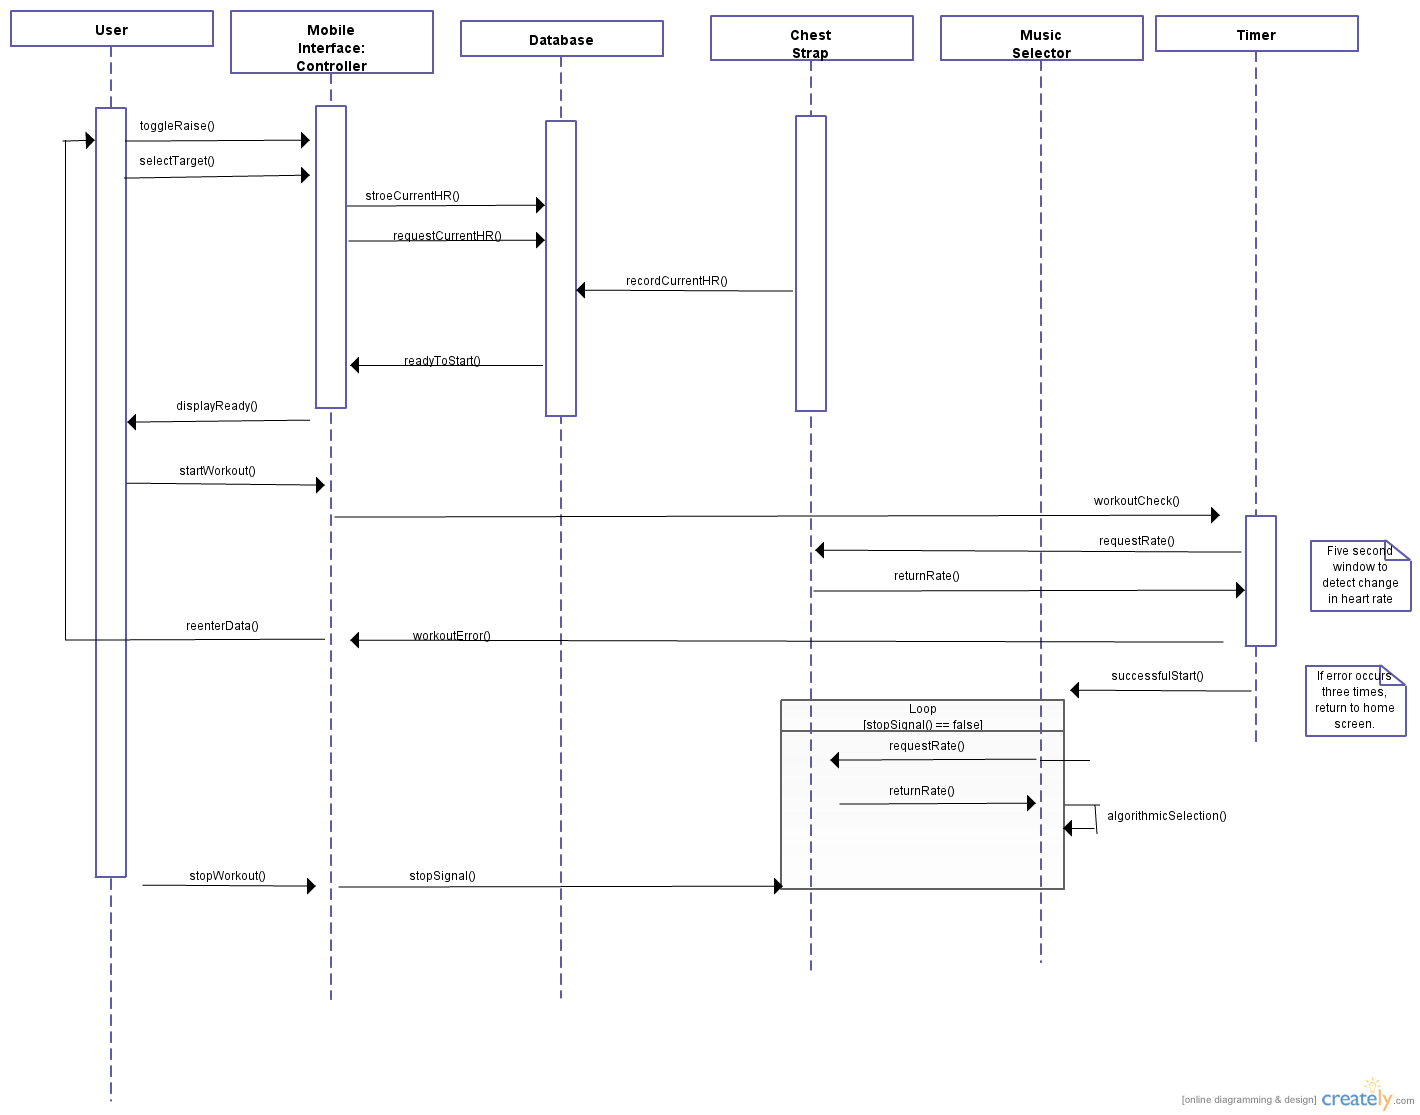
\includegraphics[scale=.35]{img/Interaction_Diagrams/newUC1.png}\\
    \caption {Interaction diagram for the increaseHeartRate case} 
\end{figure}


Since our first two use cases are very similar, we only include the interaction diagram for UC-1, increaseHeartRate. Again, the user toggles the ``raise'' button from the home screen and scrolls to the desired BPM. The database manager coordinates with the heart rate monitor and uses its own algorithm to determine the appropriate song for the music player to play for the user. Then, it waits five seconds for the user to begin his workout. Upon playback, the database manager continuously receives the user's current BPM and makes adjustments to the song's tempo accordingly.

\begin{figure}[H]
    \centering
    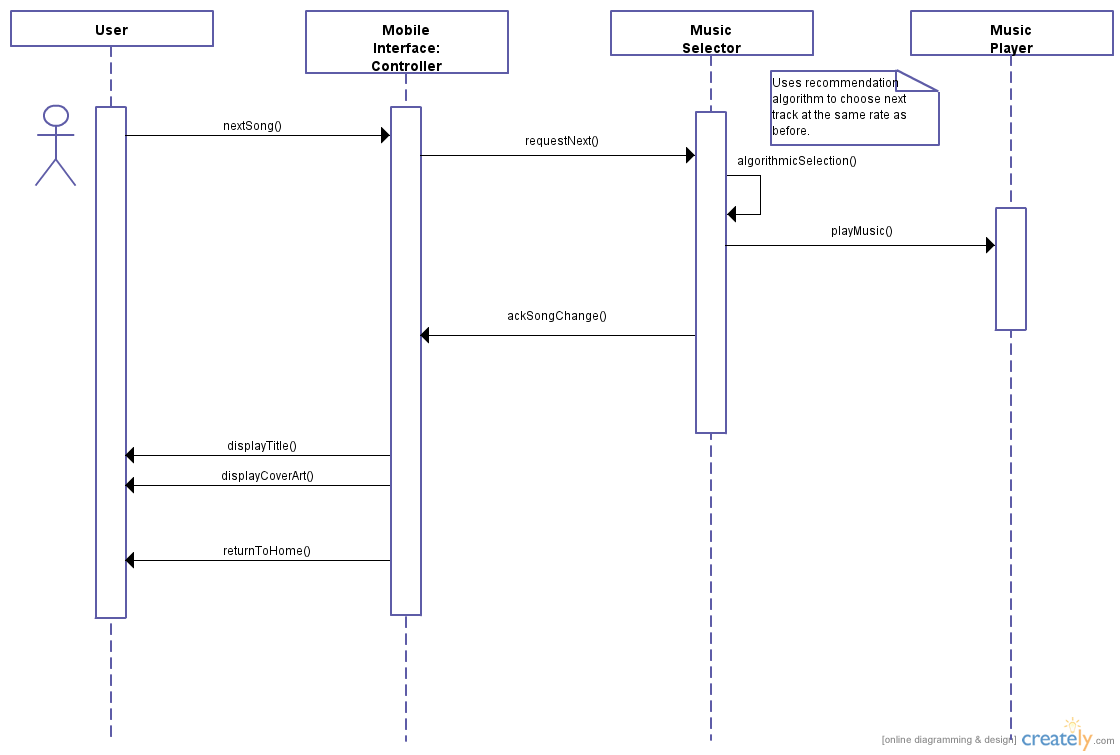
\includegraphics[scale=.40]{img/Interaction_Diagrams/newUC3.png}\\
    \caption {Interaction diagram for getNextSong()} 
\end{figure}

For our third use case, the user's goal is to listen to another song. Similar to the ``skip'' button on most standard music players, we included a double fast-forward arrow for users' convenience. When pressed, the controller immediately contacts the database manager. The database manager selects another track based on its song-selection algorithm for the music player to play. (If the user is currently trying to change his/her heart rate, the database manager will take that into count and select a song of a similar speed.) It also returns the cover art and new song title for the mobile interface to display.

\begin{figure}[H]
    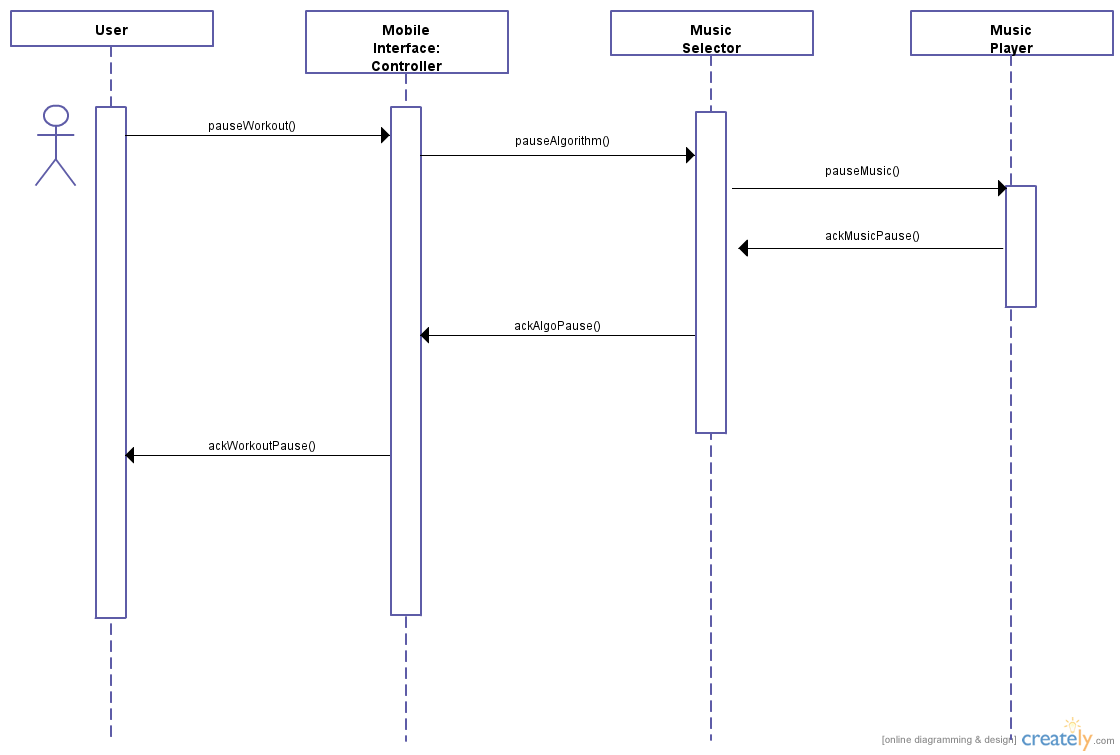
\includegraphics[scale=.40]{img/Interaction_Diagrams/newUC4.png}\\
    \caption {Interaction diagram for pausePlayback()} 
\end{figure}

Our pausePlayback sequence is fairly simple. The user initiates the request by tapping the play/pause button. Then the controller informs the database manager to store the current state settings for future use, and the database manager proceeds to stop recording data and allows the music player to stop the song. The mobile display also updates accordingly.

\begin{figure}[H]
    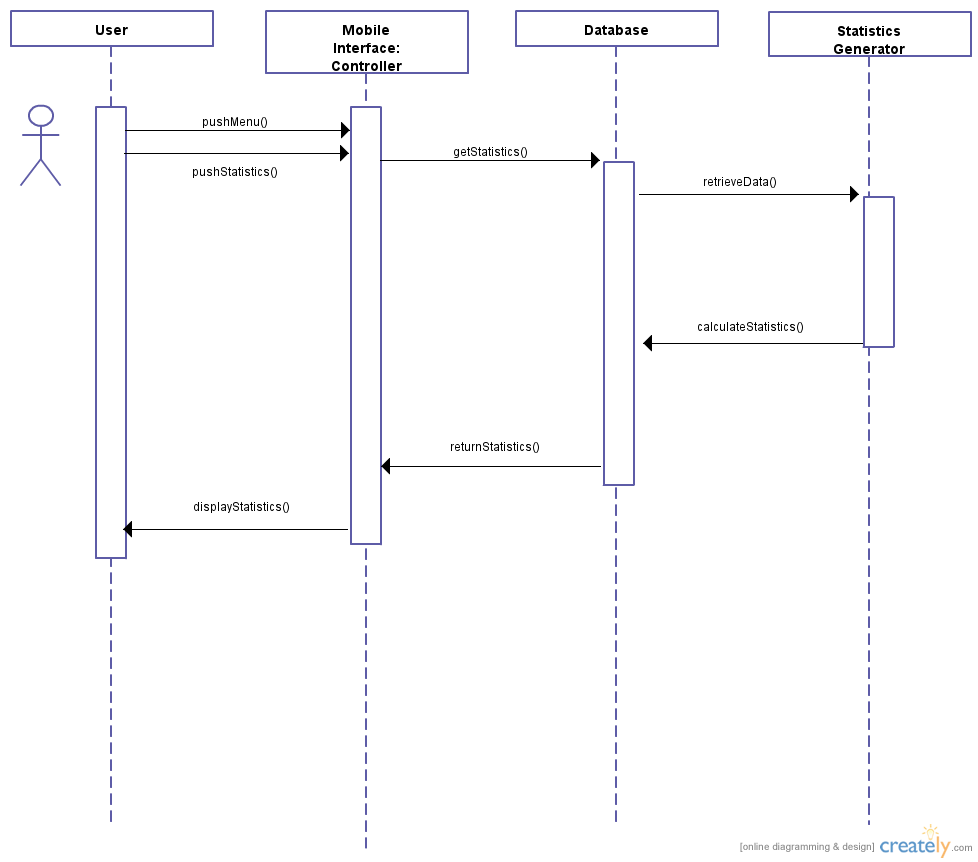
\includegraphics[scale=.40]{img/Interaction_Diagrams/newUC5.png}\\
    \caption {Interaction diagram for getStatistics()} 
\end{figure}
In UC-5, getStatistics, the user begins with two button presses to achieve their goal. First, they bring up the menu button in the top right hand corner and then press ``Statistics'' from the dropdown. The controller passes this request to the database manager, which quickly retrieves and updates the data. Then, it calculates statistics, creates some graphs, and then returns the output to the controller to display. (Note that the user must select from the options available in order to view his workout history.)

\begin{figure}[H]
    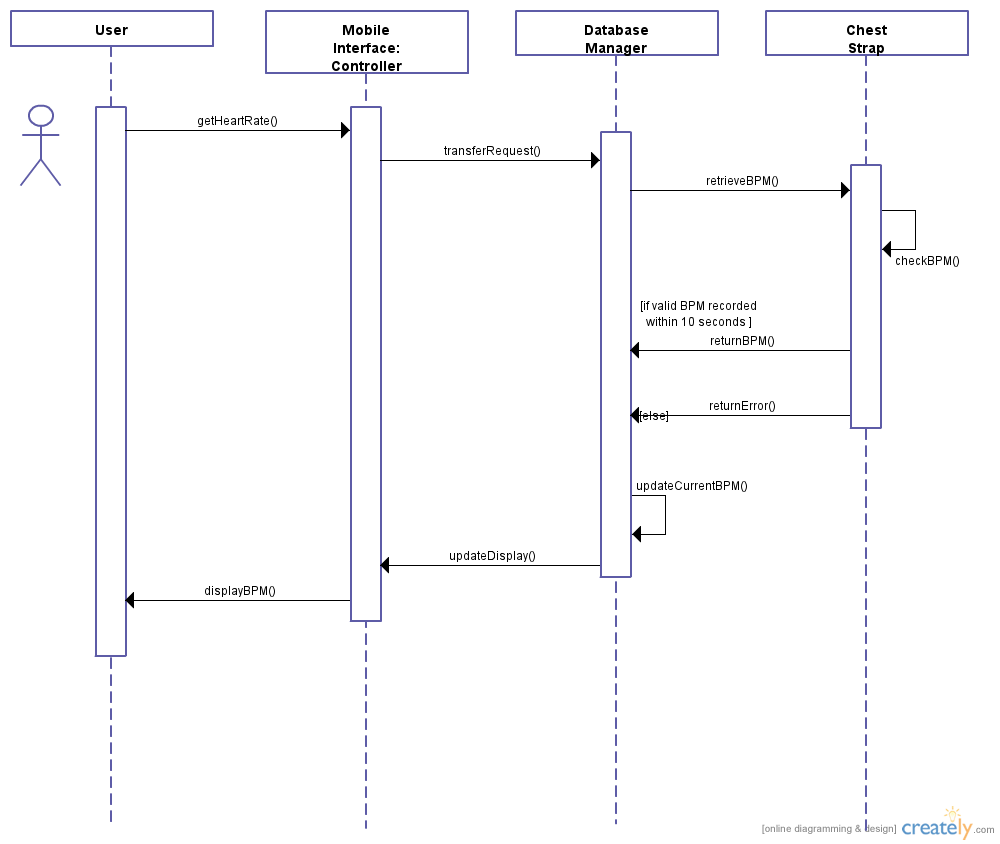
\includegraphics[scale=.40]{img/Interaction_Diagrams/newUC6.png}\\
    \caption {Interaction diagram for getHeartRate()} 
\end{figure}

UC-6, getHeartRate is very similar to UC-5. This use case is also applicable for UC-1, because the Heart Rate is important, needing to be determined continuously. The controller takes the request from the user and passes it to the database manager to handle. The database manager then takes the current BPM value from the Heart Rate Monitor and updates the value for the mobile interface to display to the user. 


\section{Alternate Scenarios}
\begin{figure}[H]
    \centering
    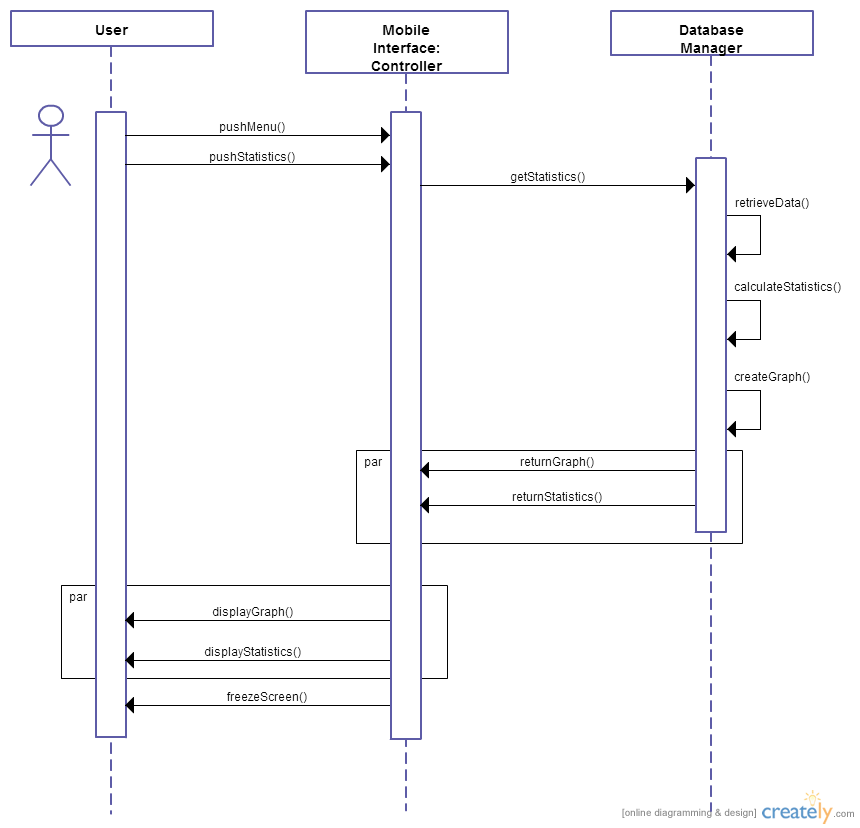
\includegraphics[scale=.30]{img/Interaction_Diagrams/UC-5_getStatistics.png}\\
    \caption {Alternate interaction diagram for getStatistics without the Statistics Generator Object}
    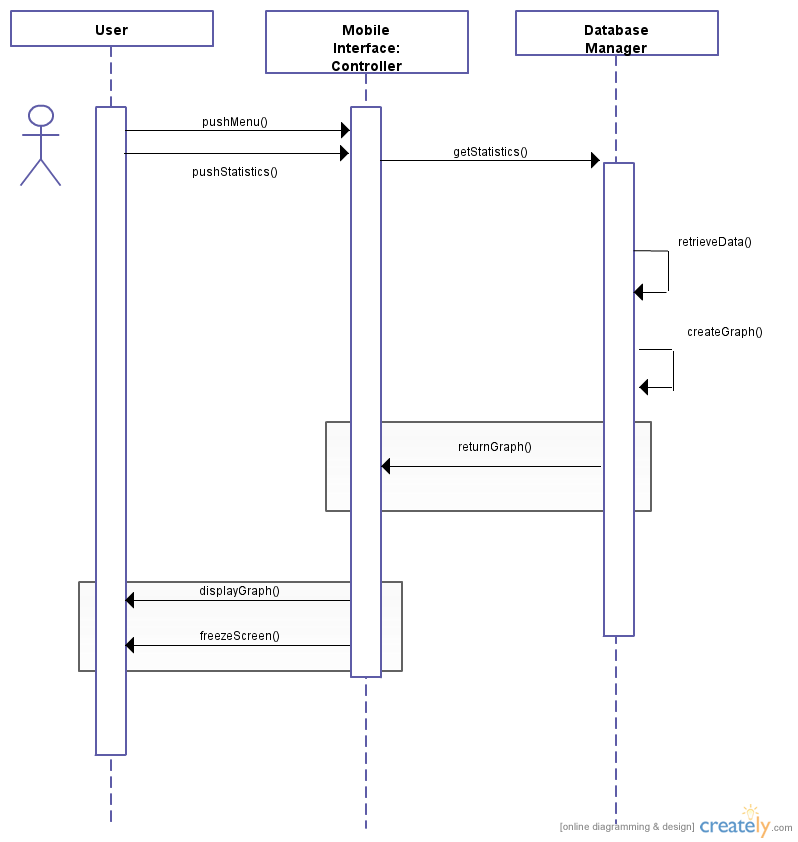
\includegraphics[scale=.30]{img/Interaction_Diagrams/getStatisticsAlternateGraphs.png}\\
    \caption {Alternate interaction diagram for getStatistics() using getGraphs()} 
\end{figure}

\begin{figure}[H]
    \centering
    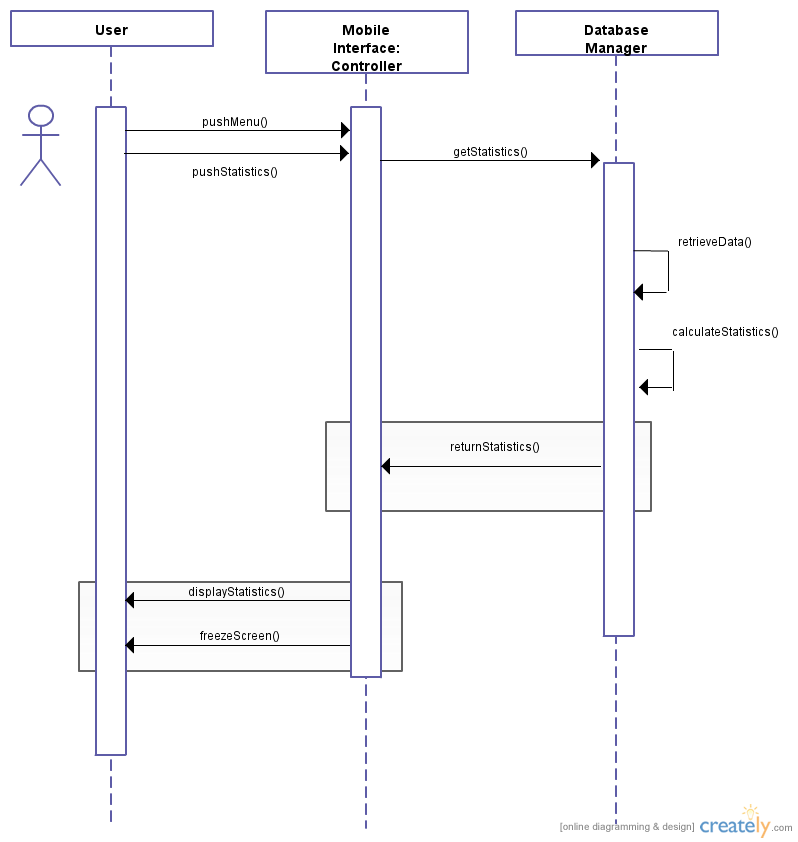
\includegraphics[scale=.30]{img/Interaction_Diagrams/getStatisticsAlternateNumbers.png}\\
    \caption {Alternate interaction diagram for getStatistics() using calculateStatistics()} 
\end{figure}




Alternate scenarios could occur mainly during the getStatistics() use case. Here, the user can select which particular graphs or data he may want to see. In the original diagram, a dedicated Statistics Generator object was created to handle the organization and creation of all statistics. This object greatly simplifies the displayStatistics() case because all the calculations are done outside of the database. However, this is not the only way to solve the case, with the alternative solution being that the statistics are generated directly by the database. Advantages of this are that there is no need to transfer the data between two objects and worry about the communication scheme between them. Also, the time needed to flesh out an entirely new class to handle the calculations would be eliminated. Three different scenarios of keeping the statistics-generation functionality are displayed above. In these diagrams, it is assumed that the user has selected all the options available for getStatistics(), and thus all the graphs and statistics available to the database are displayed to the user. This may not always be the case, as some users may prefer to see graphs only, or numbers only. Some users would like to see a certain combination of both. Thus, our alternate scenarios for the getStatistics() consist of various combinations of all the different display options. For simplicity, only the cases for displaying only graphs and for displaying only numbers are shown in separate interaction diagrams. 

Although keeping the statistics-generation functionality can be contained entirely within the database, we implemented it within a Statistics Generator object. This decision was made to keep consistency with the High Cohesion and Low Coupling Principles. If we hadn`t made the separation, then the database would have too many responsibilities to take care of. By creating a dedicated Statistics Generator object, the statistics can be fully fleshed out and managed without having to worry about other responsibilities.

\section{Design Patterns}

This project was developed through a mainly object-oriented approach. We were able to boil our system down to a few, distinct actors, and an object-oriented approach seemed appropriate to model our system. As evidenced by the interaction diagrams, there are five main actors: the user, the mobile interface, the database, the music player, and the heart rate monitor. Each of these actors has a specific set of actions that they can perform, and these actions are not very tightly coupled to those of other actions in the system. For example, the music player is designated to solely play the music on the device. It does not have access to the music algorithm or the heart rate; its sole job is to respond to requests about playing or pausing the music. Similarly, the database manager is solely responsible for manipulating data and handling requests. These characteristics are prime examples of the High Cohesion principles, because each actor in the system has its own specific tasks, and the respective actors are designed to that their tasks are carried out very well. We acknowledge that some of the actors are more important than the others, such as the database manager and the mobile interface, but this is out of necessity. The user interacts directly with the interface, and the interface talks directly to the database in most cases. The other objects in the system are more supplementary in the sense that they carry out the commands given to them by the database-mobile-interface pair. Although there is some communication between the different objects, the communication has been designed such that each method call is specific, efficient, and effective. This cuts back on unnecessary communication between the objects and allows for the system to be optimized. The Low Coupling Principle requires that objects should ``not take on too many communication responsibilities'', and our design fulfills the requirement because we have minimized the number of interactions to just the necessary ones. All in all, our object-oriented design encompasses aspects from both the High Cohesion and Low Coupling principles, and creates and effective solution to the heart rate monitoring problem.

\section{Assignment of Responsibilities}

A prime example can be found in UC-4, pausePlayback. Each object submits a request to the next object in line before reaching the Music Player, which is supposed to fulfill the ``pause'' function. At this point, the interactions start coming back. It is clearly seen that each object in this example transmits at most two messages, and no object performs more than a single computation. A similar theme exists in UC-6, getHeartRate. Each object essentially sends one message and receives one message. Furthermore, each object does not need to fulfill more than two active responsibilities. We believed that by distributing the workload for each object through the High Cohesion Principle and the Low Coupling Principle, we would be reaching the best balance.
The Expert Doer Principle was not followed as closely because the communication links of the objects we used are a bit longer. In our design, the ``one who knows'' often passes on the knowledge to another object that ``needs to know'' before the task is actually fulfilled. For instance, the Database Manager often causes the Controller to update the display and show the user rather than directly communicating with the user. Basically, our Controller and Database Manager are both extremely important, so oftentimes, they both end up with most of the implementation details.